\documentclass[xcolor={dvipsnames}]{beamer} % dvipsnames gives more built-in colors
\mode<presentation>

\usetheme{Boadilla}

\definecolor{GWdarkblue}{HTML}{033C5A}

\usecolortheme[named=GWdarkblue]{structure}

% Sets the font
\usepackage[defaultfam,tabular,lining]{montserrat}
% Capital case titles
\setbeamerfont{title}{shape=\scshape}
\setbeamerfont{frametitle}{shape=\scshape}

%Remove "Figure" from captions
\setbeamertemplate{caption}{\raggedright\insertcaption\par}

\usepackage{graphicx}
\usepackage{hyperref}

\title[Introduction]{Introduction to Data Analysis}
\author[SMPA 2152]{Data Analysis for Journalism and Political Communication (Spring 2025)}
\date{Prof. Bell}

\begin{document}

%%%%%%%%%%%%%%%%%%%%%%%%%%%%%%%%%%%%%%%%%%%%%%%%%%%%%%%%%%%%%%%%%%
\frame{
    \titlepage
}

%%%%%%%%%%%%%%%%%%%%%%%%%%%%%%%%%%%%%%%%%%%%%%%%%%%%%%%%%%%%%%%%%%

\frame{\frametitle{Expectations}
\begin{itemize}
    \item \textbf{An A effort}: Starts homework early and asks questions/attends office hours; reviews the professor's feedback; reads assignment instructions and grading rubrics carefully; attends class; being perfect at coding is not an expectation of an A effort.
    \item \textbf{A B effort}: Completes all homework assignments; does not carefully read assignment instructions; uses outside resources to complete the homework; attends class; a B effort meets minimum expectations.
    \item \textbf{A C effort or lower}: Does not complete all homework assignments; does not carefully read assignment instructions; does not communicate with the professor; does not consistently attend class; I will reach out if you meet these criteria.
\end{itemize}
}

%%%%%%%%%%%%%%%%%%%%%%%%%%%%%%%%%%%%%%%%%%%%%%%%%%%%%%%%%%%%%%%%%%

\frame{\frametitle{When You Get Stuck}
\begin{enumerate}
    \item Look back at the lecture materials. Everything required to complete the homework is in the lecture materials.
    \item Google the error (this is different than Googling ``how do I do X?'').
    \item Email the professor. Be sure to include enough code in your email that I can recreate the problem. 
\end{enumerate}
}

%%%%%%%%%%%%%%%%%%%%%%%%%%%%%%%%%%%%%%%%%%%%%%%%%%%%%%%%%%%%%%%%%%
\frame{
    \frametitle{Chalabi: 3 Ways to Spot a Bad Statistic}
    \centering
    \href{https://www.ted.com/talks/mona_chalabi_3_ways_to_spot_a_bad_statistic}{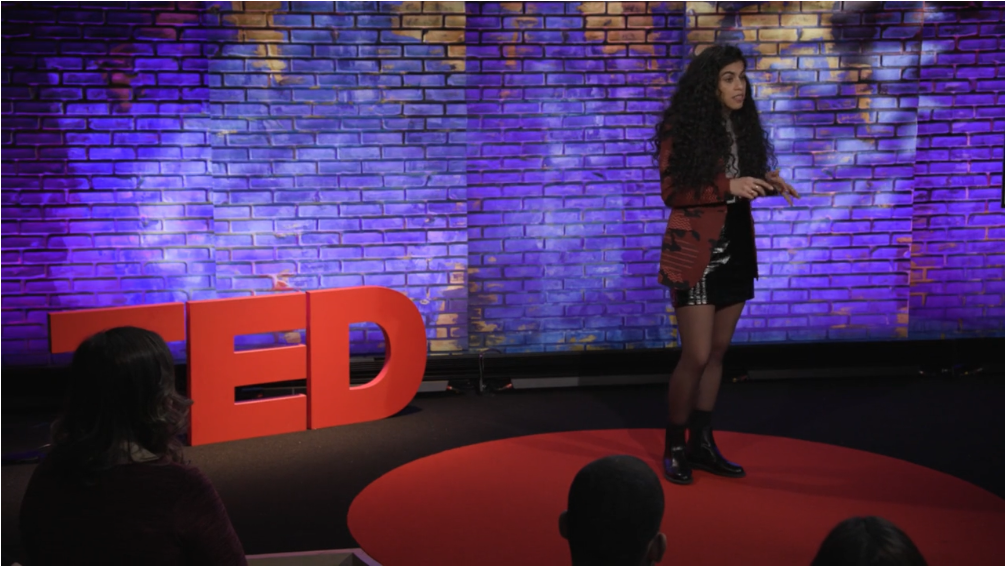
\includegraphics[height = .6\textheight]{chalabi-ted-talk.png}}
    
    \pause
    \begin{enumerate}
        \item Can you see uncertainty?
        \item Can we look beyond the averages?
        \item How was the data collected?
    \end{enumerate}
}

%%%%%%%%%%%%%%%%%%%%%%%%%%%%%%%%%%%%%%%%%%%%%%%%%%%%%%%%%%%%%%%%%%
\frame{
    \frametitle{Can you see the uncertainty?}
    \begin{itemize}[<+->]
        \item We rarely get a complete count of everything
        \item How do we know that the \textbf{sample} we choose is a good representative of the whole \textbf{population}?
        \item We will learn how to measure and communicate about uncertainty, which is both art and science
        \item Humans do not do well with probability \\
            \only<5>{
                \begin{center}
                    \begin{minipage}{.8\textwidth}
                        \begin{block}{}
                            ``There are only five probabilities the average human can handle: 99 percent, one percent, 100 percent, zero, and 50-50. That's it.'' \\ - Richard Thaler, Nobel Laureate in Economics
                        \end{block}
                    \end{minipage}
                \end{center}
            }
            \only<6>{
                
\includegraphics[height = .35\textwidth]{dc_lottery.png}
            } 
            \only<7>{
                ~\\
                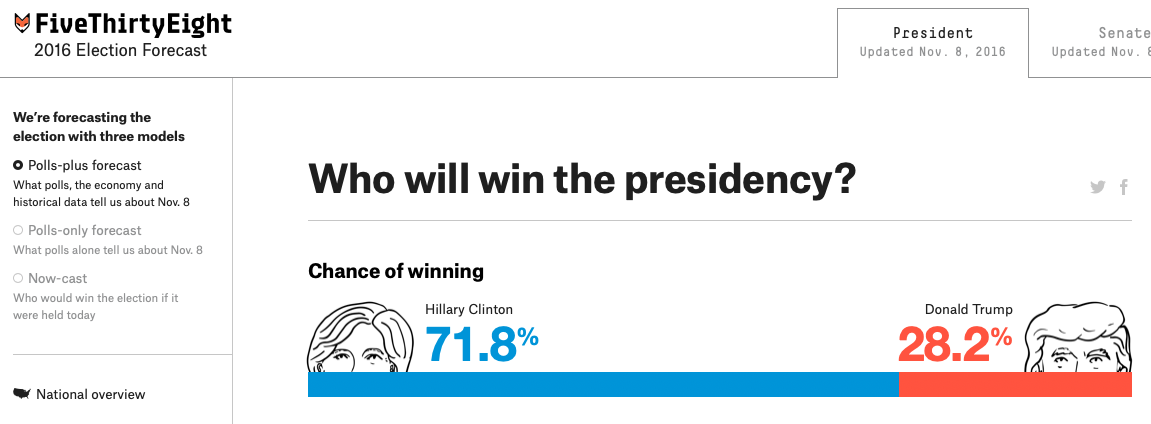
\includegraphics[height = .30\textwidth]{538_2016ElectionForecast.png}
            }
            \only<8>{
                ~\\
                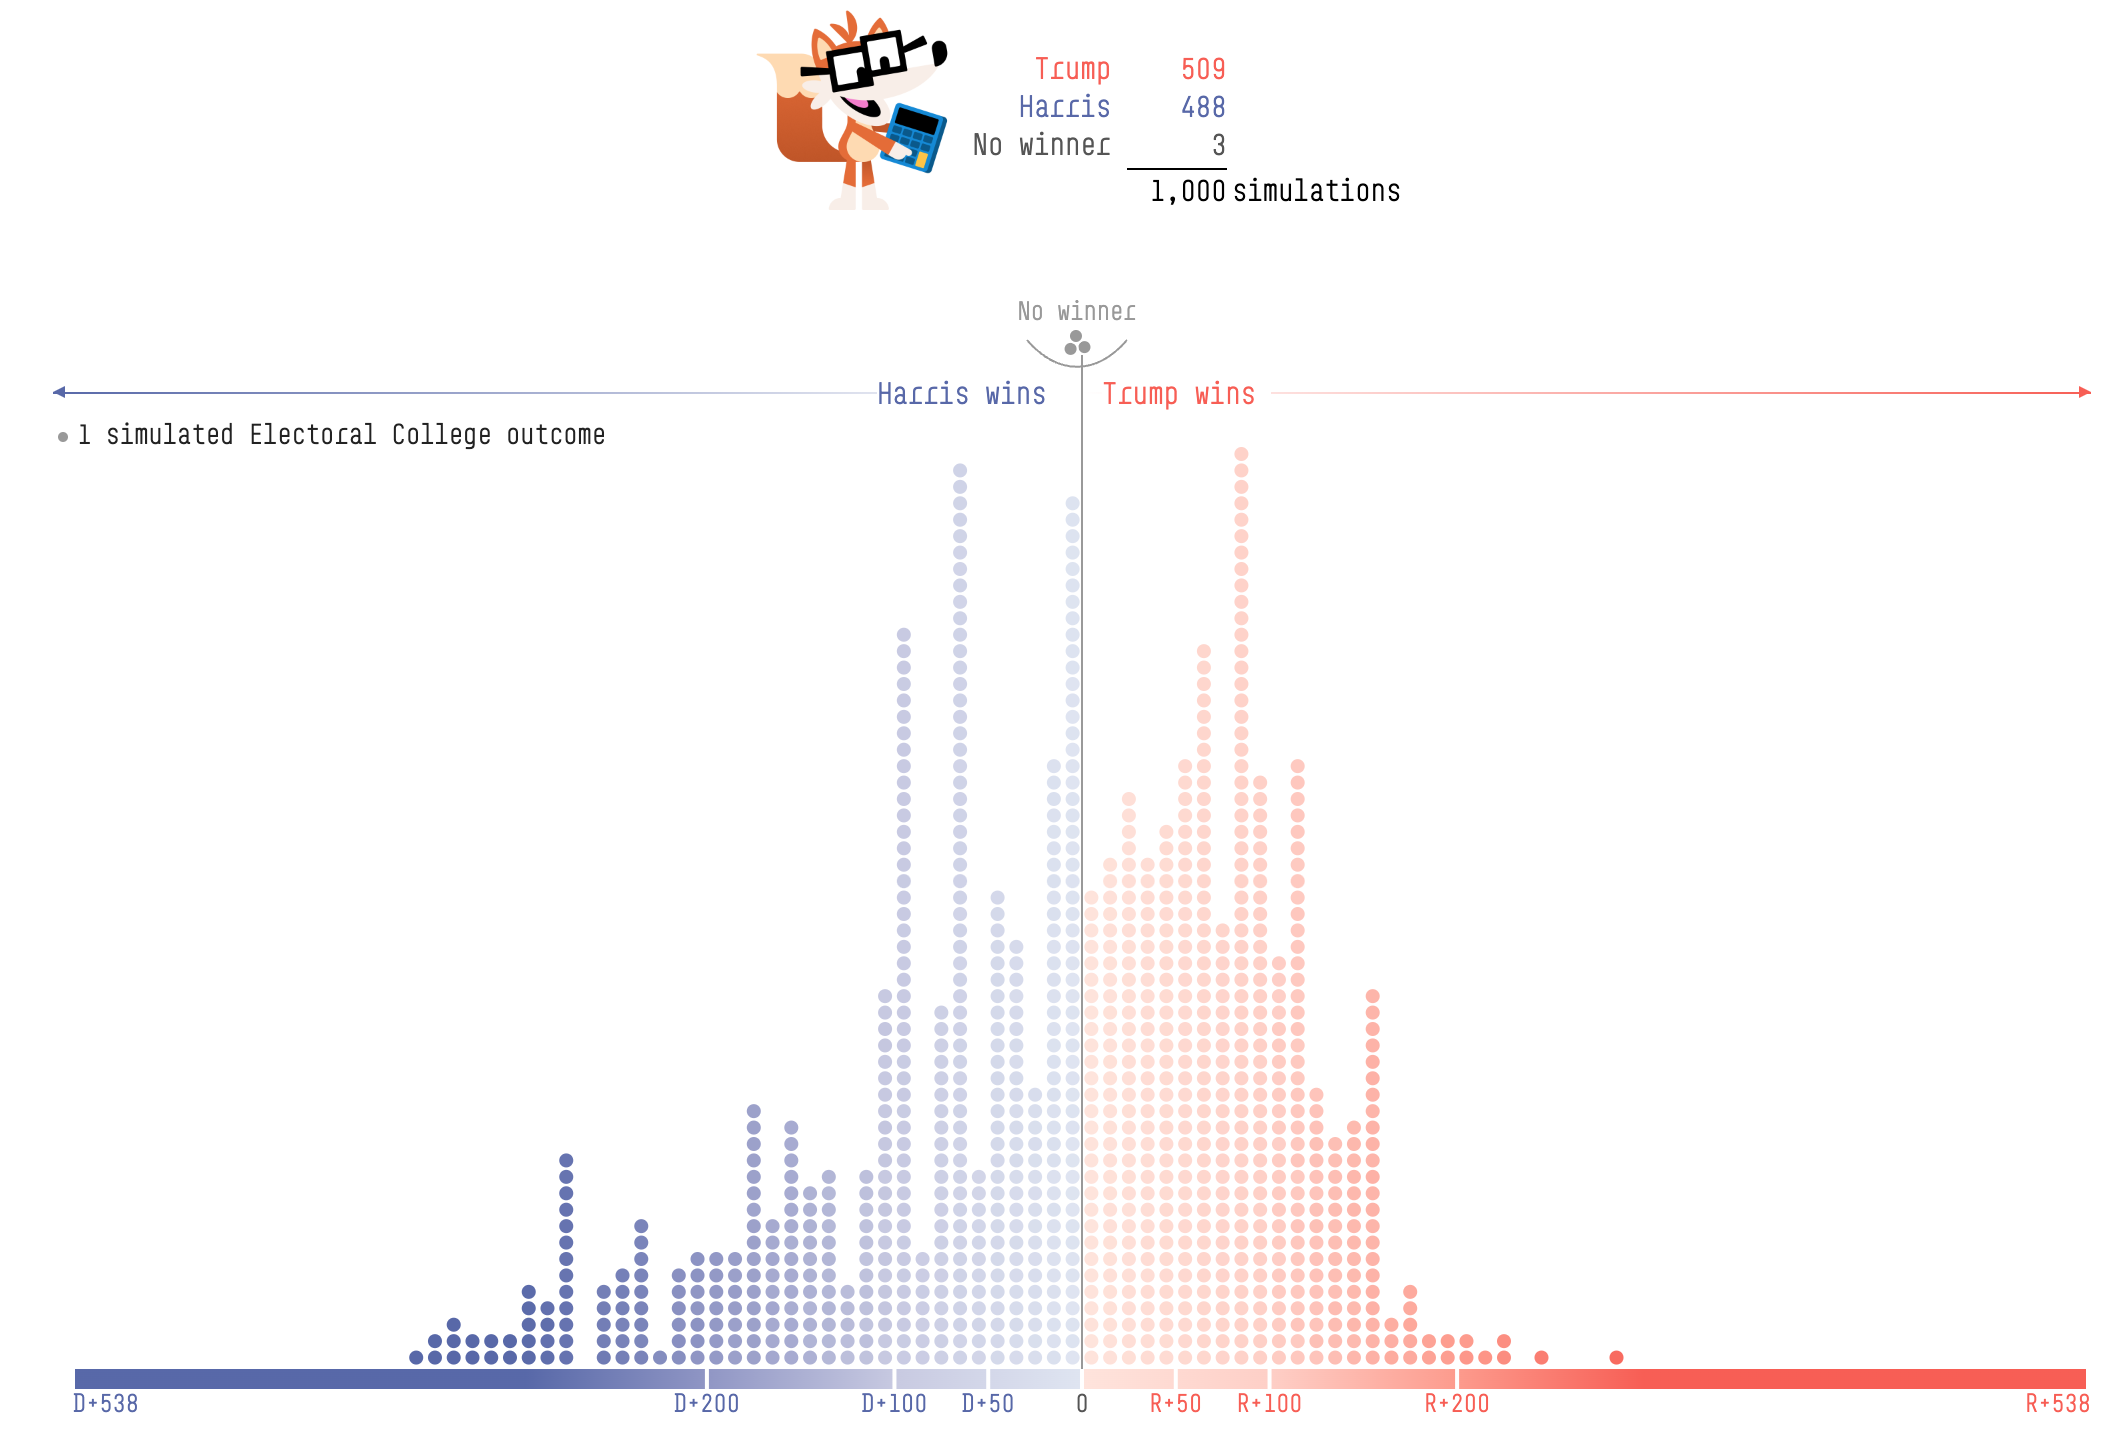
\includegraphics[height = .35\textwidth]{fivethirtyeight_30oct.png}
            }
            \only<9>{
                ~\\
                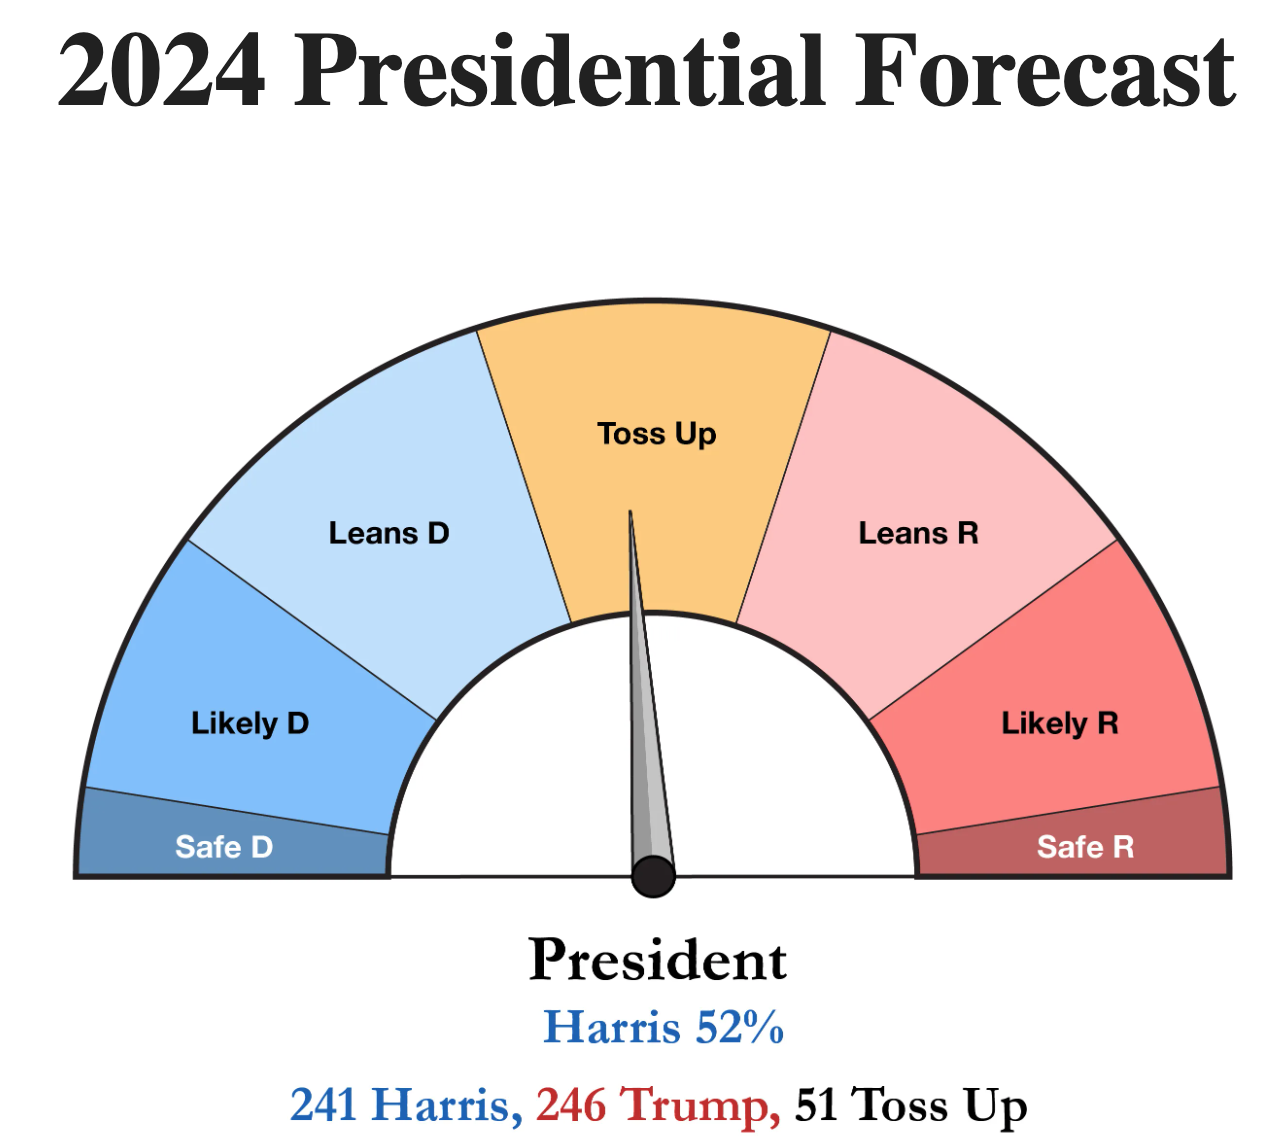
\includegraphics[height = .35\textwidth]{split_ticket_30oct.png}
            }
    \end{itemize}
}

%%%%%%%%%%%%%%%%%%%%%%%%%%%%%%%%%%%%%%%%%%%%%%%%%%%%%%%%%%%%%%%%%%
\frame{
    \frametitle{Can we look beyond the averages?}
    \only<1-2,4-5>{
        \begin{itemize}[<+->]
            \item There is always a trade-off between accuracy and simplicity when working with data
            \item We aggregate data to make it easier to comprehend, but we may also lose important context
            \item<4-> We will talk about using data visualization to communicate about data, as well as researcher choices and biases
            \item<5-> We will also talk about the importance of theory in understanding data, especially correlation vs. causation \\
            ~\\
            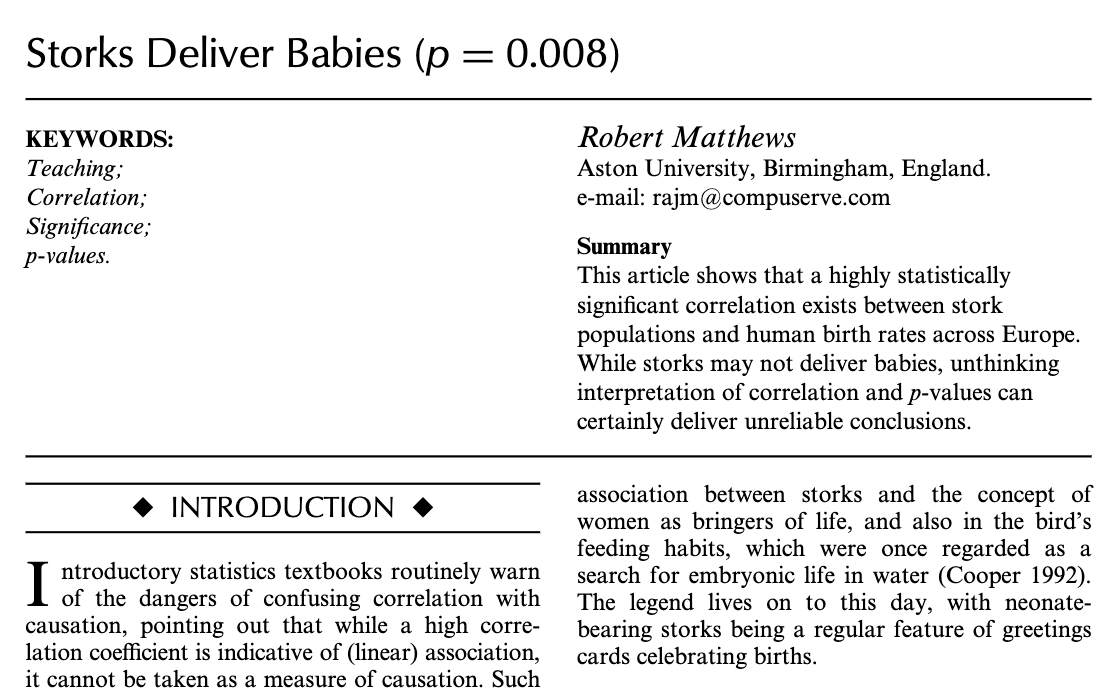
\includegraphics[height = .3\textheight]{storks.png}
        \end{itemize}
    }
    \only<3>{
        \centering
        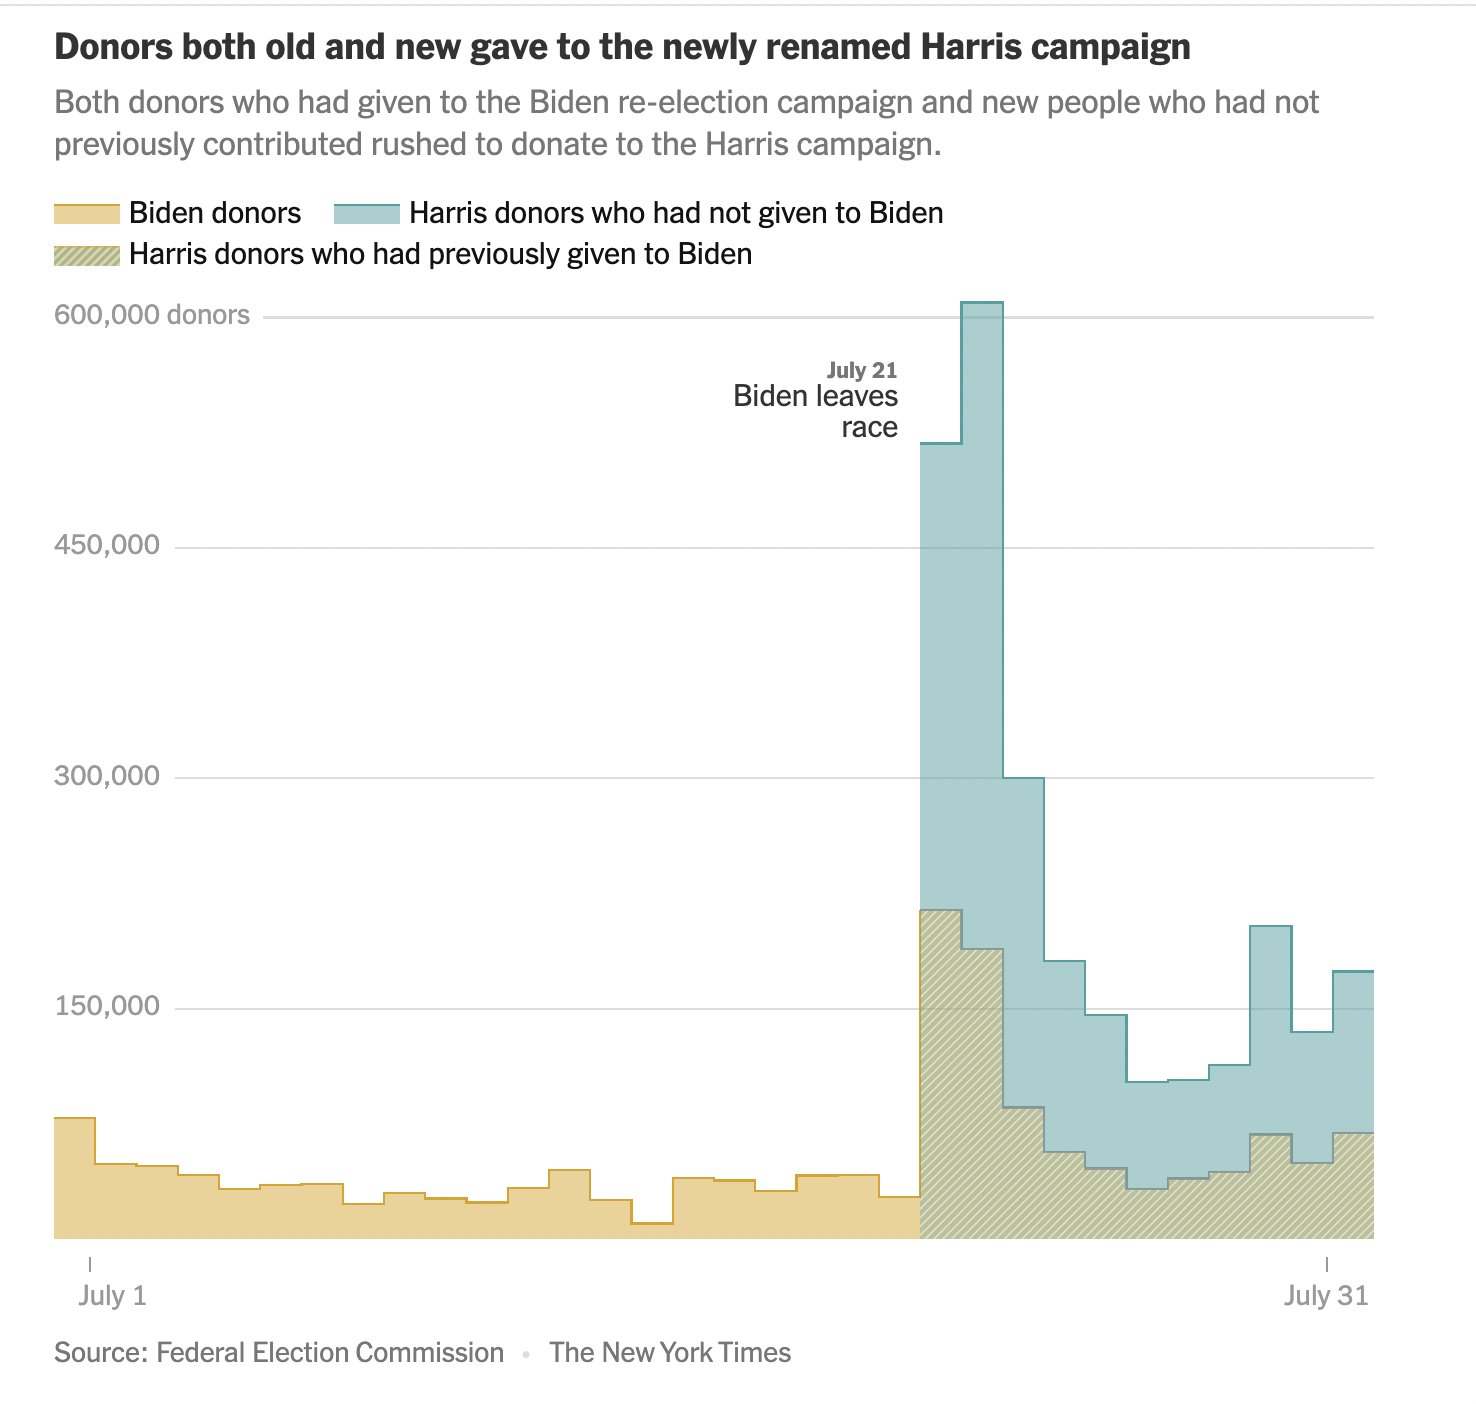
\includegraphics[height = .8\textheight]{harris_donors.jpeg}
    }
}

%%%%%%%%%%%%%%%%%%%%%%%%%%%%%%%%%%%%%%%%%%%%%%%%%%%%%%%%%%%%%%%%%%
\frame{
    \frametitle{How was the data collected?}
    \only<1-4>{
        \begin{itemize}[<+->]
            \item<1-4> Data is not objective -- it is generated by humans
            \item<2-4> Some data is produced by unscrupulous actors \\
                \only<2>{~\\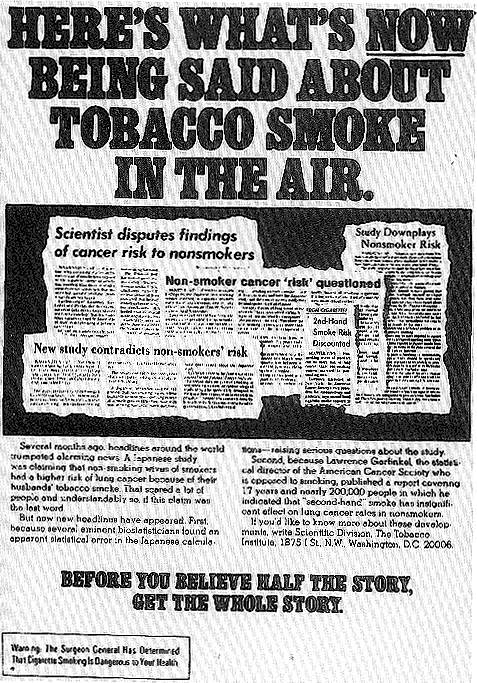
\includegraphics[height = .6\textheight]{tobacco_institute.png}}
                \only<3-4>{~\\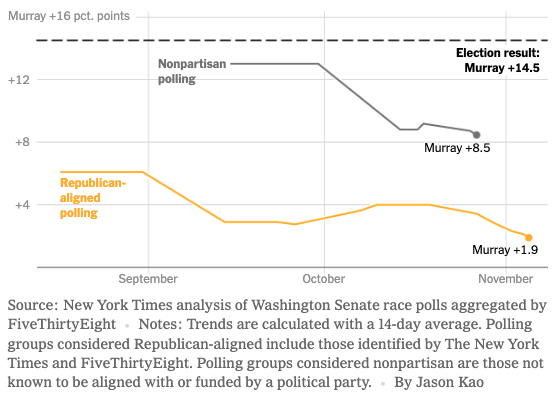
\includegraphics[height = .6\textheight]{patty_murray.png}}
            \item<4> But most of the time, poor analysis is not nefarious -- humans are imperfect
        \end{itemize}
    }
    \only<5-6, 8>{
        \begin{itemize}
            \item<5-> Garbage in = garbage out: no amount of statistical wizardry can compensate for bad data
            \item<6-> We will spend a lot of time thinking about the \textbf{data generating process} and how it can bias our results
            \item<8-> We will also discuss our ethical responsibilities around data
        \end{itemize}
    }
    \only<7>{
        \centering
        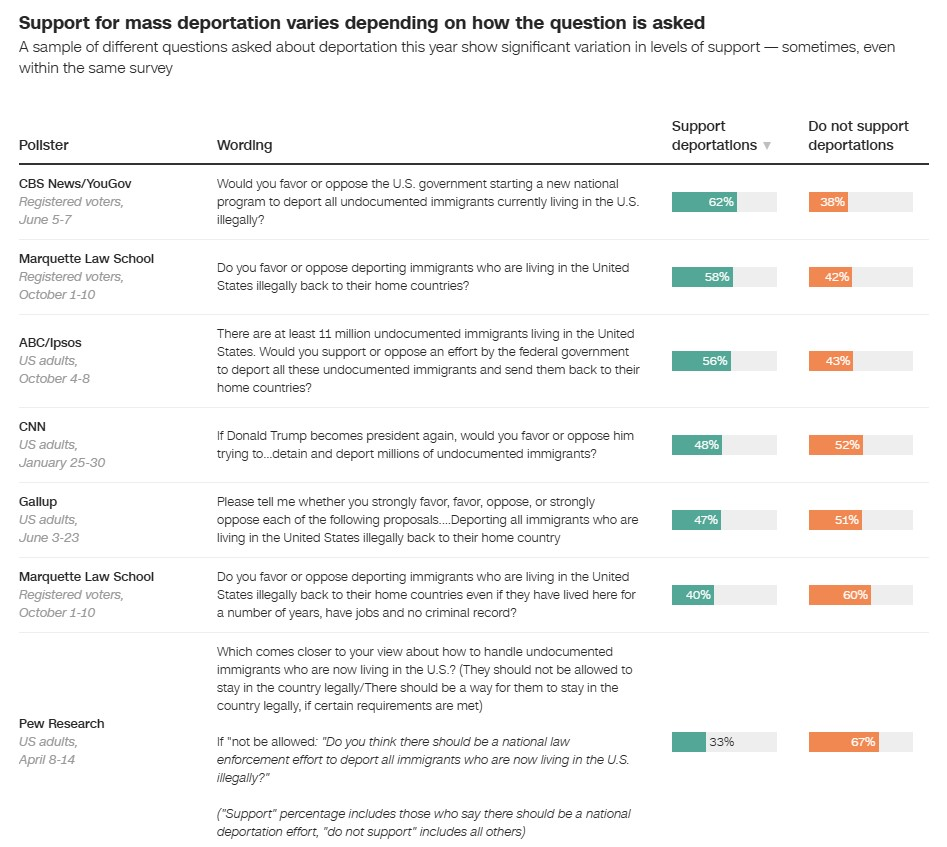
\includegraphics[height = .8\textheight]{poll_questions.jpeg}
    }
    \only<9>{
        \centering
        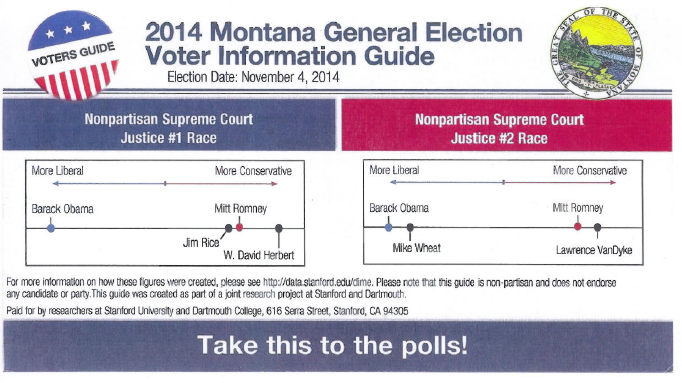
\includegraphics[width = .9\textwidth]{montana_experiment.png}
    }
}

%%%%%%%%%%%%%%%%%%%%%%%%%%%%%%%%%%%%%%%%%%%%%%%%%%%%%%%%%%%%%%%%%%
\frame{
    \frametitle{Group Discussion}
    Introduce yourself to your neighbor(s) and take a few minutes to review these additional graphs from Mona Chalabi. Do any of these stand out to you as being good (or bad) examples of our three questions for spotting a bad statistic?
    \begin{enumerate}
        \item Can you see uncertainty?
        \item Can we look beyond the averages?
        \item How was the data collected?
    \end{enumerate}
}

%%%%%%%%%%%%%%%%%%%%%%%%%%%%%%%%%%%%%%%%%%%%%%%%%%%%%%%%%%%%%%%%%%
\frame{
    On your notecard, please write:
    \begin{enumerate}
        \item Preferred name
        \item Preferred pronouns
        \item Year in school and major
        \item Your background in coding and/or statistics
        \item One thing you hope to get out of this class
    \end{enumerate}
}

\end{document}
